\section{Overview}

This tutorial extends on the node and fossil calibration tutorial and focuses on relaxed clock methods. 
In the first part we will use an uncorrelated lognormal (UCLN) relaxed clock model.
%In the second analysis you will use informative node- and fossil-calibrations instead of the informative prior on the root age.
%In the third analysis you will use minimum and maximum age constraint (both using hard and soft constraints) to calibrate the phylogeny.
All the assumptions will be covered more in detail later in this tutorial.

\subsection*{Requirements}
We assume that you have read and hopefully completed the following tutorials:
\begin{itemize}
\item RB\_Getting\_Started
\item RB\_Basics\_Tutorial
\item RB\_CTMC\_Tutorial
\item RB\_DivergenceTime\_Tutorial
\end{itemize}
Note that the RB\_Basics\_Tutorial introduces the basic syntax of \Rev but does not cover any phylogenetic models.
You may skip the RB\_Basics\_Tutorial if you have some familiarity with \R.
We tried to keep this tutorial very basic and introduce all the language concepts on the way.
You may only need the RB\_Basics\_Tutorial for a more in-depth discussion of concepts in \Rev.


%%%%%%%%
%%   Data   %%
%%%%%%%%
\section{Data and files}\label{Sec:data}

We provide the data file of DNA sequences required for this tutorial.
You may want to use your own data instead.

\noindent \\ \impmark Create a folder called \cl{data} and download the following files:
\begin{itemize}
\item \href{http://rawgit.com/revbayes/revbayes_tutorial/master/RB_DivergenceTimeRelaxedClock_Tutorial/data/primates_cytb.nex}{\cl{primates\_cytb.nex}}: Alignment of the \textit{cytochrome b} subunit from 23 primates representing 14 of the 16 families (\textit{Indriidae} and \textit{Callitrichidae} are missing).
\end{itemize}
Additionally, we will use the same fossil calibration as in the previous tutorial.




\newpage
\FloatBarrier
\section{Divergence time estimation using uncorrelated, lognormal distributed branch rates}\label{sec:UCLN}

\bigskip
\subsection{Getting Started}


The first section of this exercise involves:
(1) setting up a general time reversible (GTR) substitution model \citep{Tavare1986} with gamma distributed rate variation among sites \citep{Yang1994a} for an alignment of the cytochrome b subunit;
(2) use node calibrations to date the phylogeny;
(3) use a relaxed clock model;
(4) approximating the posterior probability of the tree topology and node ages (and all other parameters) using MCMC, and; 
(5) summarizing the MCMC output by computing the maximum \textit{a posteriori} tree. 
This analysis is mostly equivalent to the analysis performed in the RB\_CTMC\_Tutorial.

\begin{figure}[h!]
\centering
\fbox{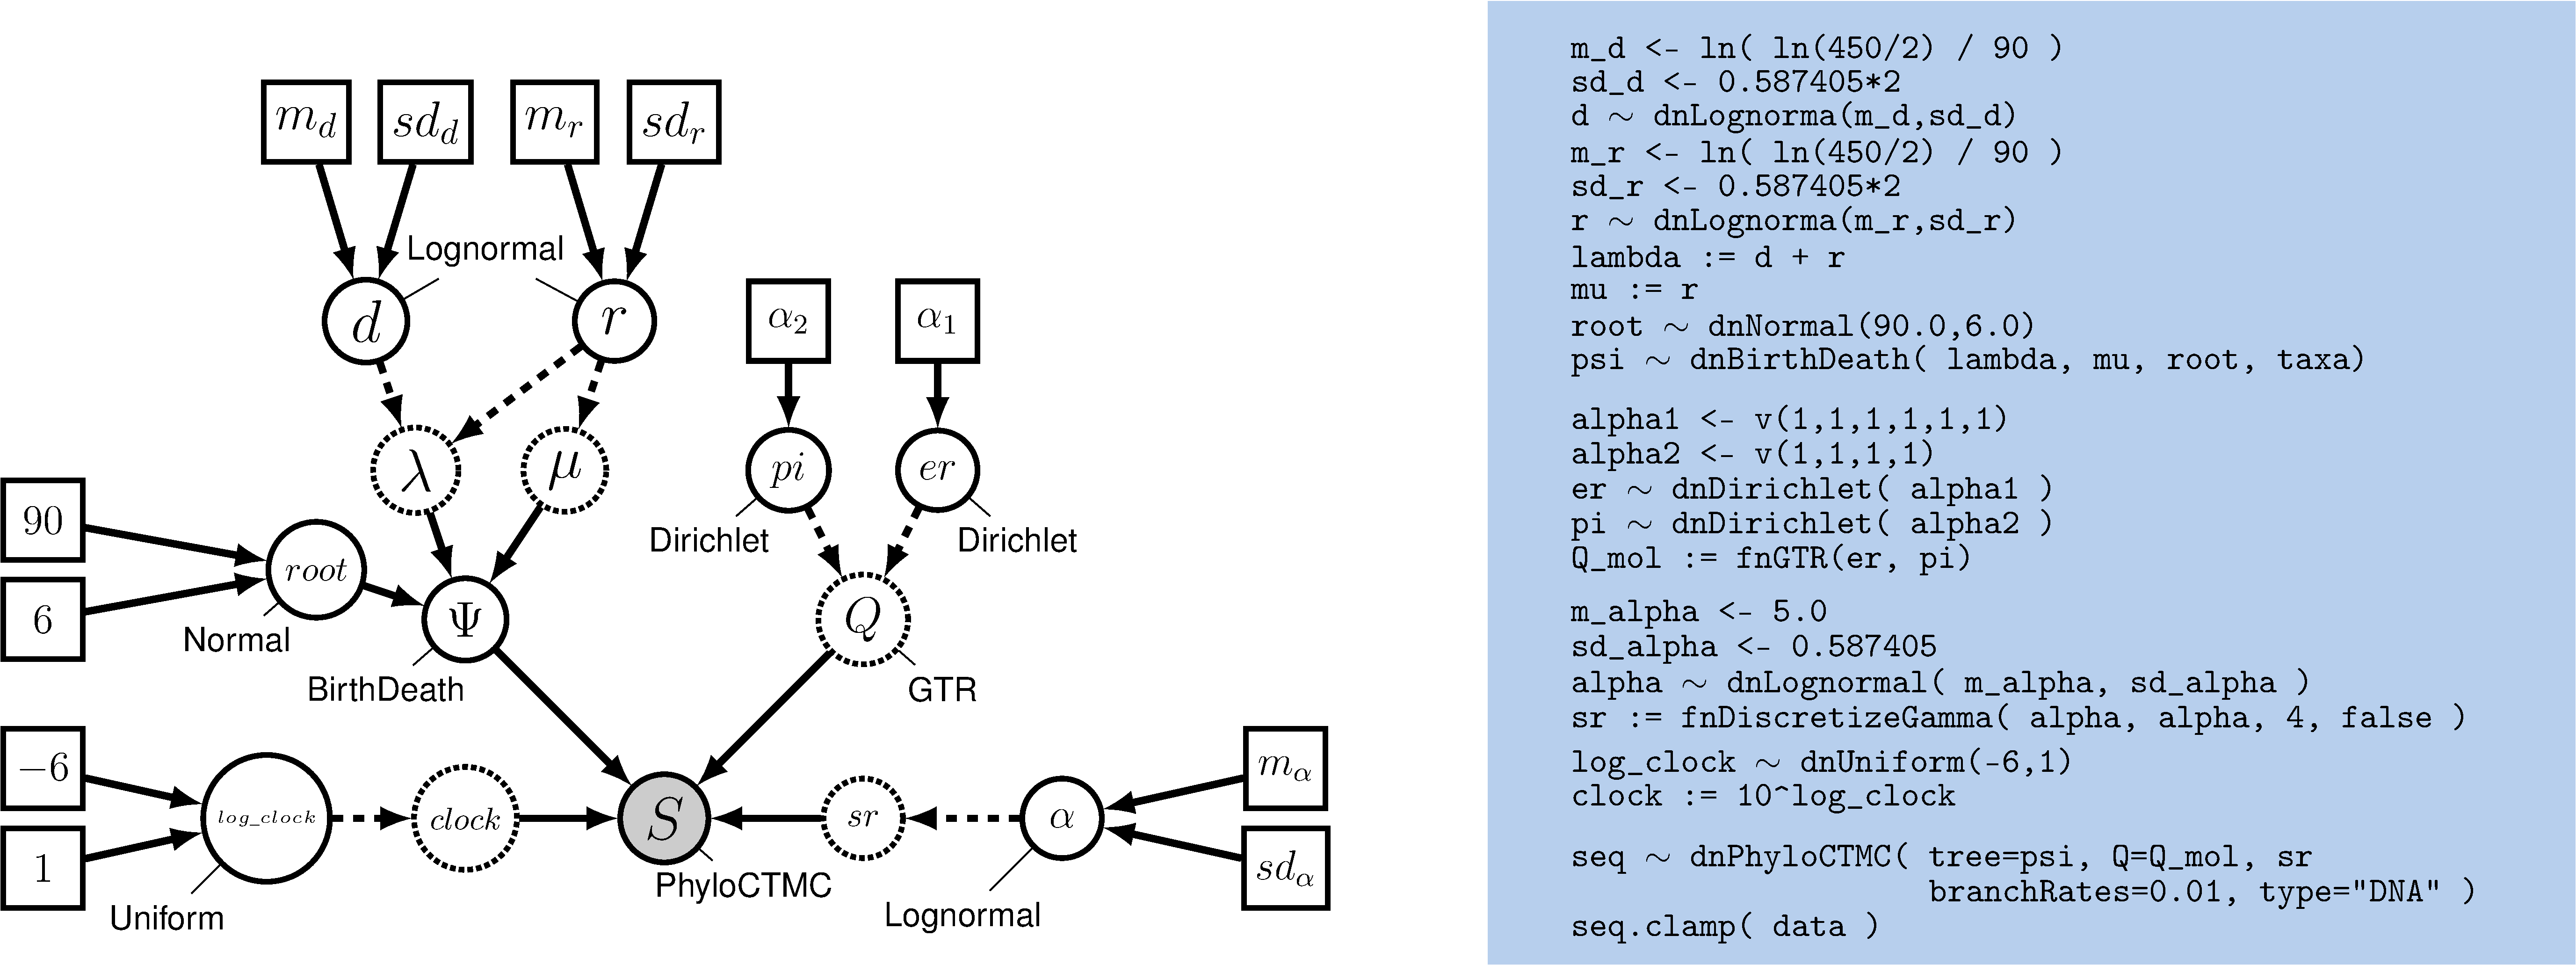
\includegraphics[width=\textwidth,angle=0]{\ResourcePath figures/root_calibration.pdf}}
\caption{\small An example phylogenetic model depicted in graphical-model notation (left) and the corresponding specification in the \Rev language (right).
This example shows the basic outline of the root calibration that we will use in the first exercise.}
\label{fig:clock_prior}
\end{figure}

The general structure of the model is represented in Figure~\ref{fig:clock_prior}.
This figure shows the full model graph.


\bigskip

\subsection{Loading the Data}

\noindent \\ \impmark You should have already downloaded the data files in Section \ref{Sec:data}. 
Links to additional files, including the scripts to run these analyses can be found on the \href{http://revbayes.github.io/tutorials.html}{\RevBayes tutorials website}. 
Remember that the data file should be in a directory called \cl{data} that is in your current working directory.

First load in the sequences using the \cl{readDiscreteCharacterData()} function. 
{\tt \begin{snugshade*}
\begin{lstlisting}
data <- readDiscreteCharacterData("data/primates_cytb.nex")
\end{lstlisting}
\end{snugshade*}}
Executing these lines initializes the data matrix as the respective \Rev variable. 

Next we will specify some useful variables based on our dataset. 
The variable \cl{data} has \textit{member functions} that we can use to retrieve information about the dataset. 
These include the number of species (\cl{n\_species}) and the tip labels (\cl{taxa}).
Each of these variables will be necessary for setting up different parts of our model (\EG the birth-death process prior).
{\tt \begin{snugshade*}
\begin{lstlisting}
n_species <- data.ntaxa()
taxa <- data.taxa()	
\end{lstlisting}
\end{snugshade*}}

Additionally, we set up a counter variable for the number of moves that we already added to our analysis.
[Recall that moves are algorithms used to propose new parameter values during the MCMC simulation.]
This will make it much easier if we extend the model or analysis to include additional moves or to remove some moves.
{\tt \begin{snugshade*}
\begin{lstlisting}
mvi = 0 
\end{lstlisting}
\end{snugshade*}}
You may have noticed that we used the \cl{=} operator to create the move index.
This simply means that the variable is not part of the model.
You will later see that we use this operator more often, \EG when we create moves and monitors.

With the data loaded, we can now proceed to specify our substitution model.



\subsection{General Time Reversible (GTR) Substitution Model}

The GTR model requires that we define and specify a prior on the six exchangeability rates, which we will describe using a flat Dirichlet distribution.
As we did previously for the Dirichlet prior on base frequencies, we first define a constant node specifying the vector of concentration-parameter values using the \cl{v()} function:
{\tt \begin{snugshade*}
\begin{lstlisting}
er_prior <- v(1,1,1,1,1,1) 
\end{lstlisting}
\end{snugshade*}}
This node defines the concentration-parameter values of the Dirichlet prior distribution on the exchangeability rates. 
Now, we can create a stochastic node for the exchangeability rates using the \cl{dnDirichlet()} function, which takes the vector of concentration-parameter values as an argument and the \cl{\rbdn} operator. 
Together, these create a stochastic node named \cl{er}, see Figure~\ref{fig:clock_prior}: 
{\tt \begin{snugshade*}
\begin{lstlisting}
er ~ dnDirichlet(er_prior)
\end{lstlisting}
\end{snugshade*}}
The Dirichlet prior on our parameter \cl{er} creates a \href{http://en.wikipedia.org/wiki/Simplex}{\textit{simplex}} of values that sum to 1. 


For each stochastic node in our model, we must also specify a proposal mechanism if we wish to estimate that parameter. 
{\tt\small \begin{snugshade*}
\begin{lstlisting}
moves[++mvi] = mvSimplexElementScale(er) 
\end{lstlisting}
\end{snugshade*}}

We can use the same type of distribution as a prior on the 4 stationary frequencies ($\pi_A, \pi_C, \pi_G, \pi_T$) since these parameters also represent proportions. 
Specify a flat Dirichlet prior density on the base frequencies:
{\tt \begin{snugshade*}
\begin{lstlisting}
pi_prior <- v(1,1,1,1) 
pi ~ dnDirichlet(pi_prior)
\end{lstlisting}
\end{snugshade*}}

The node \cl{pi} represents the $\pi$ node in Figure~\ref{fig:clock_prior}.
Now add the simplex scale move on the stationary frequencies to the moves vector:
{\tt \small \begin{snugshade*}
\begin{lstlisting}
moves[++mvi] = mvSimplexElementScale(pi)  
\end{lstlisting}
\end{snugshade*}}

We can finish setting up this part of the model by creating a deterministic node for the GTR instantaneous-rate matrix \cl{Q}. 
The \cl{fnGTR()} function takes a set of exchangeability rates and a set of base frequencies to compute the instantaneous-rate matrix used when calculating the likelihood of our model.
{\tt \begin{snugshade*}
\begin{lstlisting}
Q := fnGTR(er,pi)
\end{lstlisting}
\end{snugshade*}}


\subsection{Setting up the Gamma Model}

Create a constant node called \cl{alpha\_prior\_mean} and a second constant node called \cl{alpha\_prior\_sd} for the lognormal prior on the gamma-shape parameter (this is represented as the constant rate parameter in Figure \ref{fig:clock_prior}):
{\tt\begin{snugshade*}
\begin{lstlisting}
alpha_prior_mean <- 5.0
alpha_prior_sd <- 0.587405
\end{lstlisting}
\end{snugshade*}}

Then create a stochastic node called \cl{alpha} with an lognormal prior (this represents the stochastic node for the $\alpha$-shape parameter in Figure \ref{fig:clock_prior}):
{\tt\begin{snugshade*}
\begin{lstlisting}
alpha ~ dnLognormal( alpha_prior_mean, alpha_prior_sd )
\end{lstlisting}
\end{snugshade*}}

The way the ASRV model is implemented involves discretizing the mean-one gamma distribution into a set number of rate categories, $k$. 
To specify this, we need a deterministic node that is a vector that will hold the set of $k$ rates drawn from the gamma distribution with $k$ rate categories. 
The \cl{fnDiscretizeGamma()} function returns this deterministic node and takes three arguments: the shape and rate of the gamma distribution and the number of categories. 
Since we want to discretize a mean-one gamma distribution, we can pass in \cl{alpha} for both the shape and rate.

Initialize the \cl{gamma\_rates} deterministic node vector using the  \cl{fnDiscretizeGamma()} function with \cl{4} bins:
{\tt \begin{snugshade*}
\begin{lstlisting}
gamma_rates := fnDiscretizeGamma( alpha, alpha, 4 )
\end{lstlisting}
\end{snugshade*}}

The random variable that controls the rate variation is the stochastic node \cl{alpha}. 
We will apply a simple scale move to this parameter.
{\tt \begin{snugshade*}
\begin{lstlisting}
moves[++mvi] = mvScale(alpha, weight=2.0)
\end{lstlisting}
\end{snugshade*}}

For more information on ASRV please read the \href{https://github.com/revbayes/revbayes_tutorial/raw/master/tutorial_TeX/RB_CTMC_Tutorial/RB_CTMC_Tutorial.pdf}{RB\_CTMC\_Tutorial}.



\subsection{Tree Prior: Tree Topology and Node Ages}

The tree ( the topology and node ages) is a stochastic node in our phylogenetic model. 
In Figure \ref{fig:clock_prior}, the tree is denoted $\Psi$.
We will assume a constant-rate birth-death process as the prior distribution on the tree.
The distribution in \RevBayes is \cl{dnBDP()}. 
For more information on tree priors please read the \href{https://github.com/revbayes/revbayes_tutorial/raw/master/tutorial_TeX/RB_DiversificationRate_Tutorial/RB_Diversification_Tutorial.pdf}{RB\_DiversificationRate\_Tutorial}.

For the birth-death process we need a speciation rate and extinction rate parameter.
Instead of prior distributions on these parameters directly, we will specify lognormal prior distributions on the diversification and turnover rates.
{\tt \begin{snugshade*}
\begin{lstlisting}
diversification_mean <- ln( ln(n_species/2.0) / 90 )
diversification_sd <- 0.587405*2
diversification ~ dnLognormal(mean=diversification_mean,sd=diversification_sd) 
moves[++mvi] = mvScale(diversification,lambda=1.0,tune=true,weight=3.0)

turnover_mean <- ln( ln(n_species/2.0) / 90 )
turnover_sd <- 0.587405*2
turnover ~ dnLognormal(mean=turnover_mean,sd=turnover_sd) 
moves[++mvi] = mvScale(turnover,lambda=1.0,tune=true,weight=3.0)

### Transform the parameters
birth_rate := diversification + turnover
death_rate := turnover
\end{lstlisting}
\end{snugshade*}}

In our reference publication, \cite{Perelman2011} used a normal distribution with mean of 90.0 MYA with stdev = 6.0 as the prior distribution on the root age.
The normal distribution itself is defined on the complete real line (\IE from $-\infty$ to $+\infty$), however, we know that the root age of primates is definitely larger than 0 (it happen before the present) and smaller than, say, 5000 MYA.
Thus, we truncate the normal distribution.
This also has the advantage that the type of the variable for the root age is a positive real number, instead of a real number.
{\tt \begin{snugshade*}
\begin{lstlisting}
root_time ~ dnNormal(mean=90.0,sd=6.0,min=0.0,max=5000.0)
moves[++mvi] = mvScale(root_time,weight=2.0)
\end{lstlisting}
\end{snugshade*}}

Additionally, we know that we do not have all primate species included in this data set.
We only have 23 out of the approximately 450 primate species.
Thus, we use a sampling fraction to represent this incomplete taxon sampling \citep{Hoehna2011,Hoehna2014a}.
{\tt \begin{snugshade*}
\begin{lstlisting}
rho <- n_species/450
\end{lstlisting}
\end{snugshade*}}

Next, specify the \cl{tree} stochastic node by passing in the tip labels \cl{taxa} to the \cl{dnBDP()} distribution:
{\tt \begin{snugshade*}
\begin{lstlisting}
psi ~ dnBDP(lambda=birth_rate, mu=death_rate, rho=rho, rootAge=root_time, samplingStrategy="uniform", condition="survival", taxa=taxa)
\end{lstlisting}
\end{snugshade*}}

Some types of stochastic nodes can be updated by a number of alternative moves. 
Different moves may explore parameter space in different ways, and it is possible to use multiple different moves for a given parameter to improve mixing (the efficiency of the MCMC simulation). 
In the case of our rooted tree, for example, we can use both a nearest-neighbor interchange move without and with changing the node ages (\cl{mvNarrow} and \cl{mvNNI}) and a fixed-nodeheight subtree-prune and regrafting move (\cl{mvFNPR}). 
For overviews about moves on tree see \cite{Lakner2008}, \cite{Hoehna2008} and \cite{Hoehna2012}.
We also need moves that change the ages of the internal nodes; which are for example the \cl{mvSubtreeScale} and \cl{mvNodeTimeSlideUniform}.
These moves do not have tuning parameters associated with them, thus you only need to pass in the \cl{psi} node and proposal \cl{weight}. 
{\tt \begin{snugshade*}
\begin{lstlisting}
moves[++mvi] = mvNarrow(psi, weight=5.0)
moves[++mvi] = mvNNI(psi, weight=1.0)
moves[++mvi] = mvFNPR(psi, weight=5.0)
moves[++mvi] = mvFNPR(psi, weight=2.0)
moves[++mvi] = mvSubtreeScale(psi, weight=3.0)
moves[++mvi] = mvNodeTimeSlideUniform(psi, weight=15.0)
\end{lstlisting}
\end{snugshade*}}
The weight specifies how often the move will be applied either on average per iteration or relative to all other moves.
Have a look at the MCMC tutorial for more details about moves and MCMC strategies: \href{http://revbayes.github.io/tutorials.html}{http://revbayes.github.io/tutorials.html}

\subsection{Calibrating node ages}

In this exercise we use soft-bounded node calibrations \citep{Yang2006}.
You can also apply different node calibrations if you want.

We start with a deterministic node monitoring the age of the \emph{Catarrhini}.
This involves create a clade object.
A clade object simply contains a number of species names.
Note, the names need to match \textbf{exactly}.
Then, we use the \cl{tmrca} function which will record the \underline{t}ime of the \underline{m}ost \underline{r}ecent \underline{c}ommon \underline{a}ncestor of this clade.
Once we have this variable, we can use it for our calibration
{\tt \begin{snugshade*}
\begin{lstlisting}
clade_catarrhini = clade("Pan_paniscus", "Macaca_mulatta")
age_catarrhini := tmrca(psi, clade_catarrhini)
min_age_catarrhini <- 20.55
max_age_catarrhini <- 37.3
width_age_prior_catarrhini <- (max_age_catarrhini-min_age_catarrhini)/2.0
mean_age_prior_catarrhini <- min_age_catarrhini + width_age_prior_catarrhini
obs_age_catarrhini ~ dnSoftBoundUniformNormal(min=age_catarrhini - width_age_prior_catarrhini, max=age_catarrhini + width_age_prior_catarrhini, sd=2.5, p=0.95)
obs_age_catarrhini.clamp( mean_age_prior_catarrhini )
\end{lstlisting}
\end{snugshade*}}

Next, a calibration for the \emph{Platyrrhini}:
{\tt \begin{snugshade*}
\begin{lstlisting}
clade_platyrrhini = clade("Alouatta_palliata", "Callicebus_donacophilus")
age_platyrrhini := tmrca(psi, clade_platyrrhini)
min_age_platyrrhini <- 11.8
max_age_platyrrhini <- 37.3
width_age_prior_platyrrhini <- (max_age_platyrrhini-min_age_platyrrhini)/2.0
mean_age_prior_platyrrhini <- min_age_platyrrhini + width_age_prior_platyrrhini
obs_age_platyrrhini ~ dnSoftBoundUniformNormal(min=age_platyrrhini - width_age_prior_platyrrhini, max=age_platyrrhini + width_age_prior_platyrrhini, sd=2.5, p=0.95)
obs_age_platyrrhini.clamp( mean_age_prior_platyrrhini )
\end{lstlisting}
\end{snugshade*}}

Then, a calibration for the \emph{Simiiformes}:
{\tt \begin{snugshade*}
\begin{lstlisting}
clade_simiiformes = clade("Cebus_albifrons", "Macaca_mulatta")
age_simiiformes := tmrca(psi, clade_simiiformes)
min_age_simiiformes <- 28.3
max_age_simiiformes <- 56
width_age_prior_simiiformes <- (max_age_simiiformes-min_age_simiiformes)/2.0
mean_age_prior_simiiformes <- min_age_simiiformes + width_age_prior_simiiformes
obs_age_simiiformes ~ dnSoftBoundUniformNormal(min=age_simiiformes - width_age_prior_simiiformes, max=age_simiiformes + width_age_prior_simiiformes, sd=2.5, p=0.95)
width_age_prior_simiiformes)
obs_age_simiiformes.clamp( mean_age_prior_simiiformes )
\end{lstlisting}
\end{snugshade*}}

And finally, a calibration for the \emph{Lorisiformes}:
{\tt \begin{snugshade*}
\begin{lstlisting}
clade_lorisiformes = clade("Loris_tardigradus", "Galago_senegalensis")
age_lorisiformes := tmrca(psi, clade_lorisiformes)
min_age_lorisiformes <- 37.1
max_age_lorisiformes <- 56
width_age_prior_lorisiformes <- (max_age_lorisiformes-min_age_lorisiformes)/2.0
mean_age_prior_lorisiformes <- min_age_lorisiformes + width_age_prior_lorisiformes
obs_age_lorisiformes ~ dnSoftBoundUniformNormal(min=age_lorisiformes - width_age_prior_lorisiformes, max=age_lorisiformes + width_age_prior_lorisiformes, sd=2.5, p=0.95)
width_age_prior_lorisiformes)
obs_age_lorisiformes.clamp( mean_age_prior_lorisiformes )
\end{lstlisting}
\end{snugshade*}}


\subsection{The Uncorrelated Lognormal Relaxed Clock Model}

In theory each branch has its own clock rate drawn independently and identically (iid) from a lognormal distribution.
However, independent draws from this continuous distribution are problematic because the prior density would converge to $\infty$ when all rates are equal and the variance is equal to zero.
Instead, a discretized version of the chosen prior distribution behaves better and is computationally more efficient.
We will thus specify (more or less arbitrarily) the number of rate categories to be 10.
{\tt \begin{snugshade*}
\begin{lstlisting}
NUM_RATE_CATEGORIES = 10
\end{lstlisting}
\end{snugshade*}}
You can experiment with the number of rate categories if you want.

The lognormal distribution is parameterized by the log-transformed mean and the standard deviation.
As usual, we will say that every magnitude or clock rates between $10^{-6}$ and $10^{1}$ are equally probably a priori.
Additionally, we use an exponential prior distribution on the standard deviation because we want to give the highest prior probability to small values which represent our preference to a more clock-like behavior.
{\tt \begin{snugshade*}
\begin{lstlisting}
ucln_mean ~ dnUnif(1E-6, 10)
ucln_log_mean := ln( ucln_mean )
ucln_sigma ~ dnExponential(10.0)
\end{lstlisting}
\end{snugshade*}}
Since both variables are stochastic parameters of the model, and defined for positive real numbers, we apply scaling moves on them.
{\tt \begin{snugshade*}
\begin{lstlisting}moves[++mvi] = mvScale(ucln_mean, lambda=0.5, weight=5.0)
moves[++mvi] = mvScale(ucln_sigma, lambda=0.5, weight=5.0)
\end{lstlisting}
\end{snugshade*}}
In the next step we use the function \cl{fnDiscretizeDistribution} to compute the quantiles deterministically of the lognormal distribution.
The \cl{fnDiscretizeDistribution} function can be applied to discretize any distribution (\EG the exponential or gamma distribution) we
{\tt \begin{snugshade*}
\begin{lstlisting}
rate_categories := fnDiscretizeDistribution(dnLnorm(ucln_log_mean, ucln_sigma), NUM_RATE_CATEGORIES)
\end{lstlisting}
\end{snugshade*}}

{\tt \begin{snugshade*}
\begin{lstlisting}
rate_probs <- simplex(rep(1, NUM_RATE_CATEGORIES))
\end{lstlisting}
\end{snugshade*}}

{\tt \begin{snugshade*}
\begin{lstlisting}
for (j in 1:n_branches) {
    # for each branch pull from one of the rate categories
    branch_rates[j] ~ dnMixture(rate_categories, rate_probs)
    moves[++mvi] = mvMixtureAllocation(branch_rates[j], weight=2.0)
}
\end{lstlisting}
\end{snugshade*}}

{\tt \begin{snugshade*}
\begin{lstlisting}
mean_rt := mean(branch_rates)
\end{lstlisting}
\end{snugshade*}}



\subsection{Putting it All Together}

We have fully specified all of the parameters of our phylogenetic model---the tree topology with branch lengths, and the substitution model that describes how the sequence data evolved over the tree with branch lengths.  
Collectively, these parameters comprise a distribution called the \textit{phylogenetic continuous-time Markov chain}, and we use the \cl{PhyloCTMC} constructor function to create this node.
This distribution requires several input arguments: 
(1) the \cl{tree} with branch lengths; 
(2) the instantaneous-rate matrix \cl{Q};
(3) the branch-specific clock rates, and; 
(4) the \cl{type} of character data.


Build the random variable for the character data (sequence alignment).
{\tt \begin{snugshade*}
\begin{lstlisting}
# the sequence evolution model
seq ~ dnPhyloCTMC(tree=psi, Q=Q, branchRates=branch_rates, siteRates=gamma_rates, type="DNA")
\end{lstlisting}
\end{snugshade*}}


Once the \cl{PhyloCTMC} model has been created, we can attach our sequence data to the tip nodes in the tree.
{\tt \begin{snugshade*}
\begin{lstlisting}
seq.clamp(data)
\end{lstlisting}
\end{snugshade*}}
Finally, we wrap the entire model to provide convenient access to the DAG. 
To do this, we only need to give the \cl{model()} function a single node. 
With this node, the \cl{model()} function can find all of the other nodes by following the arrows in the graphical model:
{\tt \begin{snugshade*}
\begin{lstlisting}
mymodel = model(Q)
\end{lstlisting}
\end{snugshade*}}

\bigskip
\subsection{Performing an MCMC Analysis Under the Global Clock Model}

In this section, will describe how to set up the MCMC sampler and summarize the resulting posterior distribution of trees. 

\subsubsection{Specifying Monitors}

For our MCMC analysis, we set up a vector of \textit{monitors} to record the states of our Markov chain. 
First, we will initialize the model monitor using the \cl{mnModel} function. 
This creates a new monitor variable that will output the states for all model parameters when passed into a MCMC function. 
{\tt \begin{snugshade*}
\begin{lstlisting}
monitors[++mni] = mnModel(filename="output/primates_cytb_UCLN.log",printgen=10, separator = TAB)
\end{lstlisting}
\end{snugshade*}}

The \cl{mnFile} monitor will record the states for only the parameters passed in as arguments. 
We use this monitor to specify the output for our sampled trees.
{\tt \begin{snugshade*}
\begin{lstlisting}
monitors[++mni] = mnFile(filename="output/primates_cytb_UCLN.trees",printgen=10, separator = TAB, psi)
\end{lstlisting}
\end{snugshade*}}

Finally, create a screen monitor that will report the states of specified variables to the screen with \cl{mnScreen}:
{\tt \begin{snugshade*}
\begin{lstlisting}
monitors[++mni] = mnScreen(printgen=1000, mean_rt, root_time, age_simiiformes)
\end{lstlisting}
\end{snugshade*}}

\subsubsection{Initializing and Running the MCMC Simulation}

With a fully specified model, a set of monitors, and a set of moves, we can now set up the MCMC algorithm that will sample parameter values in proportion to their posterior probability. 
The \cl{mcmc()} function will create our MCMC object:
{\tt \begin{snugshade*}
\begin{lstlisting}
mymcmc = mcmc(mymodel, monitors, moves)
\end{lstlisting}
\end{snugshade*}}

We may wish to run the \cl{.burnin()} member function.
{\tt \begin{snugshade*}
\begin{lstlisting}
mymcmc.burnin(generations=10000,tuningInterval=250)
\end{lstlisting}
\end{snugshade*}}

Now, run the MCMC:
{\tt \begin{snugshade*}
\begin{lstlisting}
mymcmc.run(generations=30000)
\end{lstlisting}
\end{snugshade*}}

When the analysis is complete, you will have the monitored files in your output directory.

\noindent \\ \impmark Look at the file called \cl{output/primates\_cytb\_UCLN.log} in \texttt{Tracer}.


\subsection{Exercise 1}

Again, we are interested in the divergence time estimate between \emph{Simiiformes}, \emph{Platyrrhini}, \emph{Catarrhini}, \emph{Lorisiformes} and all primates.

\begin{itemize}
\item Specify your model using the UCLN relaxed clock as outlined above.
\item Run the MCMC analysis.
\item Look at the output in \Tracer.
\item Do the node-ages fall into the calibration intervals?
\item Fill in the Table~\ref{tab:divergence_times}.
\item \textbf{*} Repeat the analysis using an exponential distribution for the branch rates.
\end{itemize}

To obtain an estimate of the divergence time we read in the tree trace and build the annotated maximum \textit{a posteriori} tree.
{\tt \begin{snugshade*}
\begin{lstlisting}
treetrace = readTreeTrace("output/primates_cytb_UCLN.trees",
                             treetype="clock")
mapTree(treetrace,"output/primates_cytb_UCLN.tree")
\end{lstlisting}
\end{snugshade*}}
\noindent \\ \impmark Look at the file called \cl{output/primates\_cytb\_UCLN.tree} in \texttt{FigTree}.


\begin{Form}
\begin{table}[h!]
\centering
\caption{\small Estimated divergence times in our primates example$^*$.}
\resizebox{\textwidth}{!}{% <------ Don't forget this %
\begin{tabular}{l c c c c c c c c c c c}
\hline
\multicolumn{1}{l}{\textbf{ }} &\multicolumn{1}{r}{\textbf{ }} & \multicolumn{2}{c}{\textbf{Primates}}  & \multicolumn{2}{c}{\textbf{Simiiformes}} & \multicolumn{2}{c}{\textbf{Platyrrhini}} & \multicolumn{2}{c}{\textbf{Catarrhini}} & \multicolumn{2}{c}{\textbf{Lorisiformes}} \\ 
\cline{3-12}
\multicolumn{1}{l}{\textbf{Clock Model}} & \multicolumn{1}{r}{\hspace{3mm}} & \multicolumn{1}{c}{\textit{Mean Estimate}} & \multicolumn{1}{c}{\textit{Credible interval}} & \multicolumn{1}{c}{\textit{Mean Estimate}} & \multicolumn{1}{c}{\textit{Credible interval}} & \multicolumn{1}{c}{\textit{Mean Estimate}} & \multicolumn{1}{c}{\textit{Credible interval}} & \multicolumn{1}{c}{\textit{Mean Estimate}} & \multicolumn{1}{c}{\textit{Credible interval}} & \multicolumn{1}{c}{\textit{Mean Estimate}} & \multicolumn{1}{c}{\textit{Credible interval}} \\ 
\hline
\ref{sec:UCLN} UCLN & \hspace{15mm} & \TextField[name=m1,backgroundcolor={.85 .85 .85},color={1 0 0},height=4ex]{}  & \TextField[name=ml2,backgroundcolor={.85 .85 .85},color={0 0 1},height=4ex]{} & \TextField[name=m3,backgroundcolor={.85 .85 .85},color={1 0 0},height=4ex]{}  & \TextField[name=ml4,backgroundcolor={.85 .85 .85},color={0 0 1},height=4ex]{} & \TextField[name=m5,backgroundcolor={.85 .85 .85},color={1 0 0},height=4ex]{}  & \TextField[name=ml6,backgroundcolor={.85 .85 .85},color={0 0 1},height=4ex]{} & \TextField[name=m7,backgroundcolor={.85 .85 .85},color={1 0 0},height=4ex]{}  & \TextField[name=ml8,backgroundcolor={.85 .85 .85},color={0 0 1},height=4ex]{} & \TextField[name=m9,backgroundcolor={.85 .85 .85},color={1 0 0},height=4ex]{}  & \TextField[name=ml10,backgroundcolor={.85 .85 .85},color={0 0 1},height=4ex]{}\\
\hline
\ref{sec:NodeCalibration} UCE & \hspace{3mm} &\TextField[name=ml11,backgroundcolor={.85 .85 .85},color={1 0 0},height=4ex]{} & \TextField[name=ml12,backgroundcolor={.85 .85 .85},color={0 0 1},height=4ex]{} & \TextField[name=m13,backgroundcolor={.85 .85 .85},color={1 0 0},height=4ex]{}  & \TextField[name=ml14,backgroundcolor={.85 .85 .85},color={0 0 1},height=4ex]{} & \TextField[name=m15,backgroundcolor={.85 .85 .85},color={1 0 0},height=4ex]{}  & \TextField[name=ml16,backgroundcolor={.85 .85 .85},color={0 0 1},height=4ex]{} & \TextField[name=m17,backgroundcolor={.85 .85 .85},color={1 0 0},height=4ex]{}  & \TextField[name=ml18,backgroundcolor={.85 .85 .85},color={0 0 1},height=4ex]{} & \TextField[name=m19,backgroundcolor={.85 .85 .85},color={1 0 0},height=4ex]{}  & \TextField[name=ml20,backgroundcolor={.85 .85 .85},color={0 0 1},height=4ex]{} \\
%\hline
%\ref{sec:HardBounds} Hard Bounds& \hspace{3mm} &\TextField[name=ml21,backgroundcolor={.85 .85 .85},color={1 0 0},height=4ex]{} & \TextField[name=ml22,backgroundcolor={.85 .85 .85},color={0 0 1},height=4ex]{} & \TextField[name=m23,backgroundcolor={.85 .85 .85},color={1 0 0},height=4ex]{}  & \TextField[name=ml24,backgroundcolor={.85 .85 .85},color={0 0 1},height=4ex]{} & \TextField[name=m25,backgroundcolor={.85 .85 .85},color={1 0 0},height=4ex]{}  & \TextField[name=ml26,backgroundcolor={.85 .85 .85},color={0 0 1},height=4ex]{} & \TextField[name=m27,backgroundcolor={.85 .85 .85},color={1 0 0},height=4ex]{}  & \TextField[name=ml28,backgroundcolor={.85 .85 .85},color={0 0 1},height=4ex]{} & \TextField[name=m29,backgroundcolor={.85 .85 .85},color={1 0 0},height=4ex]{}  & \TextField[name=ml30,backgroundcolor={.85 .85 .85},color={0 0 1},height=4ex]{}  \\
%\hline
%\ref{sec:SoftBounds} Soft Bounds & \hspace{3mm} &\TextField[name=ml31,backgroundcolor={.85 .85 .85},color={1 0 0},height=4ex]{} & \TextField[name=ml32,backgroundcolor={.85 .85 .85},color={0 0 1},height=4ex]{} & \TextField[name=m33,backgroundcolor={.85 .85 .85},color={1 0 0},height=4ex]{}  & \TextField[name=ml34,backgroundcolor={.85 .85 .85},color={0 0 1},height=4ex]{} & \TextField[name=m35,backgroundcolor={.85 .85 .85},color={1 0 0},height=4ex]{}  & \TextField[name=ml36,backgroundcolor={.85 .85 .85},color={0 0 1},height=4ex]{} & \TextField[name=m37,backgroundcolor={.85 .85 .85},color={1 0 0},height=4ex]{}  & \TextField[name=ml38,backgroundcolor={.85 .85 .85},color={0 0 1},height=4ex]{} & \TextField[name=m39,backgroundcolor={.85 .85 .85},color={1 0 0},height=4ex]{}  & \TextField[name=ml40,backgroundcolor={.85 .85 .85},color={0 0 1},height=4ex]{}  \\
\hline
{\footnotesize{$^*$you can edit this table}}\\
\end{tabular}%
}
\label{tab:divergence_times}
\end{table}
\end{Form}


\bibliographystyle{sysbio}
\bibliography{\GlobalResourcePath refs}
